% Options for packages loaded elsewhere
\PassOptionsToPackage{unicode}{hyperref}
\PassOptionsToPackage{hyphens}{url}
%
\documentclass[
]{book}
\title{Technical Report for the Development of a Values Informed Leadership Measure}
\author{Jennifer Bragger, Diego Figueiras, Renata Garcia Prieto Palacios Roji, John Kulas \& Ian Lee}
\date{2021-12-15}

\usepackage{amsmath,amssymb}
\usepackage{lmodern}
\usepackage{iftex}
\ifPDFTeX
  \usepackage[T1]{fontenc}
  \usepackage[utf8]{inputenc}
  \usepackage{textcomp} % provide euro and other symbols
\else % if luatex or xetex
  \usepackage{unicode-math}
  \defaultfontfeatures{Scale=MatchLowercase}
  \defaultfontfeatures[\rmfamily]{Ligatures=TeX,Scale=1}
\fi
% Use upquote if available, for straight quotes in verbatim environments
\IfFileExists{upquote.sty}{\usepackage{upquote}}{}
\IfFileExists{microtype.sty}{% use microtype if available
  \usepackage[]{microtype}
  \UseMicrotypeSet[protrusion]{basicmath} % disable protrusion for tt fonts
}{}
\makeatletter
\@ifundefined{KOMAClassName}{% if non-KOMA class
  \IfFileExists{parskip.sty}{%
    \usepackage{parskip}
  }{% else
    \setlength{\parindent}{0pt}
    \setlength{\parskip}{6pt plus 2pt minus 1pt}}
}{% if KOMA class
  \KOMAoptions{parskip=half}}
\makeatother
\usepackage{xcolor}
\IfFileExists{xurl.sty}{\usepackage{xurl}}{} % add URL line breaks if available
\IfFileExists{bookmark.sty}{\usepackage{bookmark}}{\usepackage{hyperref}}
\hypersetup{
  pdftitle={Technical Report for the Development of a Values Informed Leadership Measure},
  pdfauthor={Jennifer Bragger, Diego Figueiras, Renata Garcia Prieto Palacios Roji, John Kulas \& Ian Lee},
  hidelinks,
  pdfcreator={LaTeX via pandoc}}
\urlstyle{same} % disable monospaced font for URLs
\usepackage{longtable,booktabs,array}
\usepackage{calc} % for calculating minipage widths
% Correct order of tables after \paragraph or \subparagraph
\usepackage{etoolbox}
\makeatletter
\patchcmd\longtable{\par}{\if@noskipsec\mbox{}\fi\par}{}{}
\makeatother
% Allow footnotes in longtable head/foot
\IfFileExists{footnotehyper.sty}{\usepackage{footnotehyper}}{\usepackage{footnote}}
\makesavenoteenv{longtable}
\usepackage{graphicx}
\makeatletter
\def\maxwidth{\ifdim\Gin@nat@width>\linewidth\linewidth\else\Gin@nat@width\fi}
\def\maxheight{\ifdim\Gin@nat@height>\textheight\textheight\else\Gin@nat@height\fi}
\makeatother
% Scale images if necessary, so that they will not overflow the page
% margins by default, and it is still possible to overwrite the defaults
% using explicit options in \includegraphics[width, height, ...]{}
\setkeys{Gin}{width=\maxwidth,height=\maxheight,keepaspectratio}
% Set default figure placement to htbp
\makeatletter
\def\fps@figure{htbp}
\makeatother
\setlength{\emergencystretch}{3em} % prevent overfull lines
\providecommand{\tightlist}{%
  \setlength{\itemsep}{0pt}\setlength{\parskip}{0pt}}
\setcounter{secnumdepth}{5}
\usepackage{booktabs}
\ifLuaTeX
  \usepackage{selnolig}  % disable illegal ligatures
\fi
\usepackage[]{natbib}
\bibliographystyle{apalike}

\begin{document}
\maketitle

{
\setcounter{tocdepth}{1}
\tableofcontents
}
\hypertarget{introduction}{%
\chapter{Introduction}\label{introduction}}

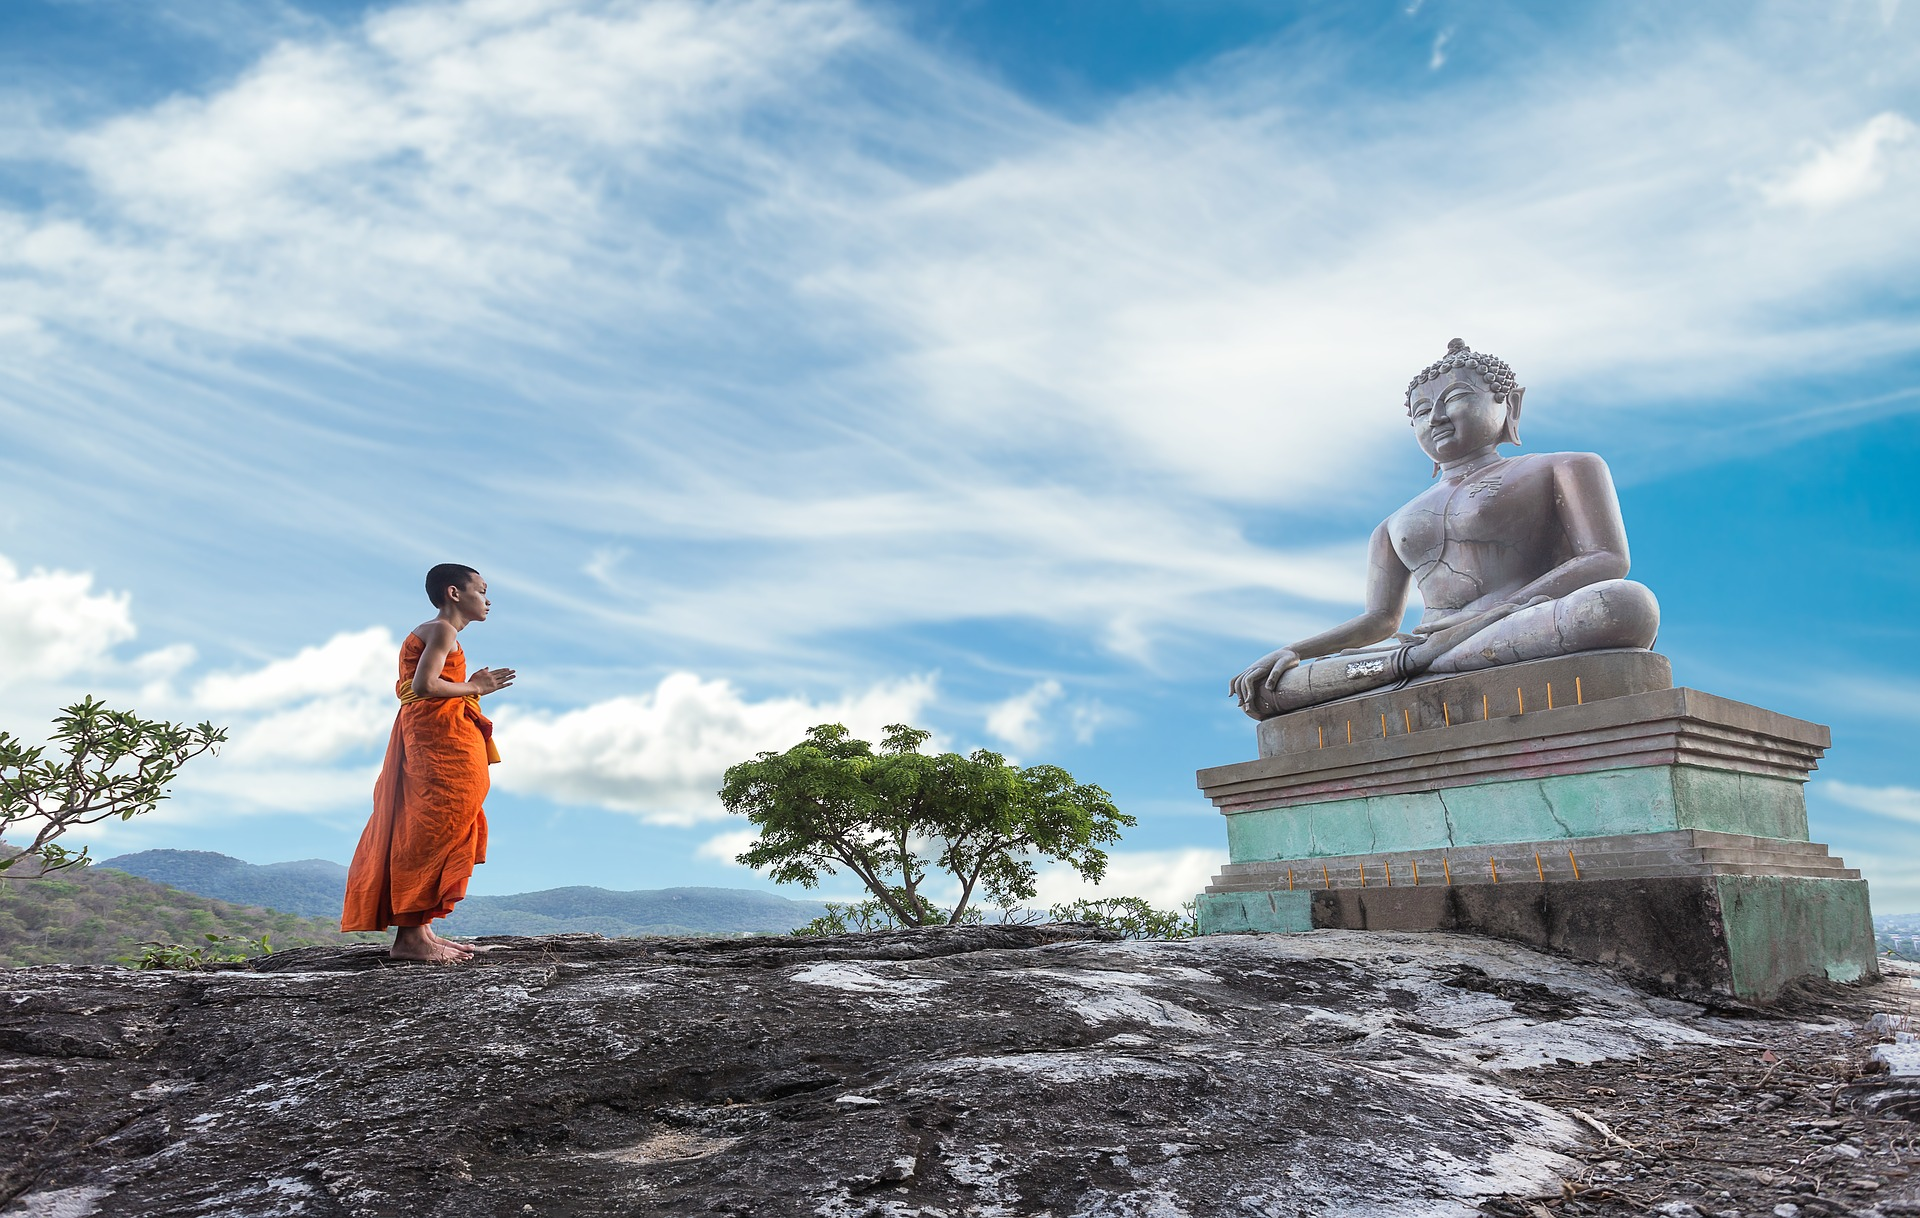
\includegraphics{monk-g0dbed9dae_1920.jpg}

This is a technical report that documents the development of a 360 assessment of effective leadership..

\hypertarget{origins}{%
\chapter{Origins}\label{origins}}

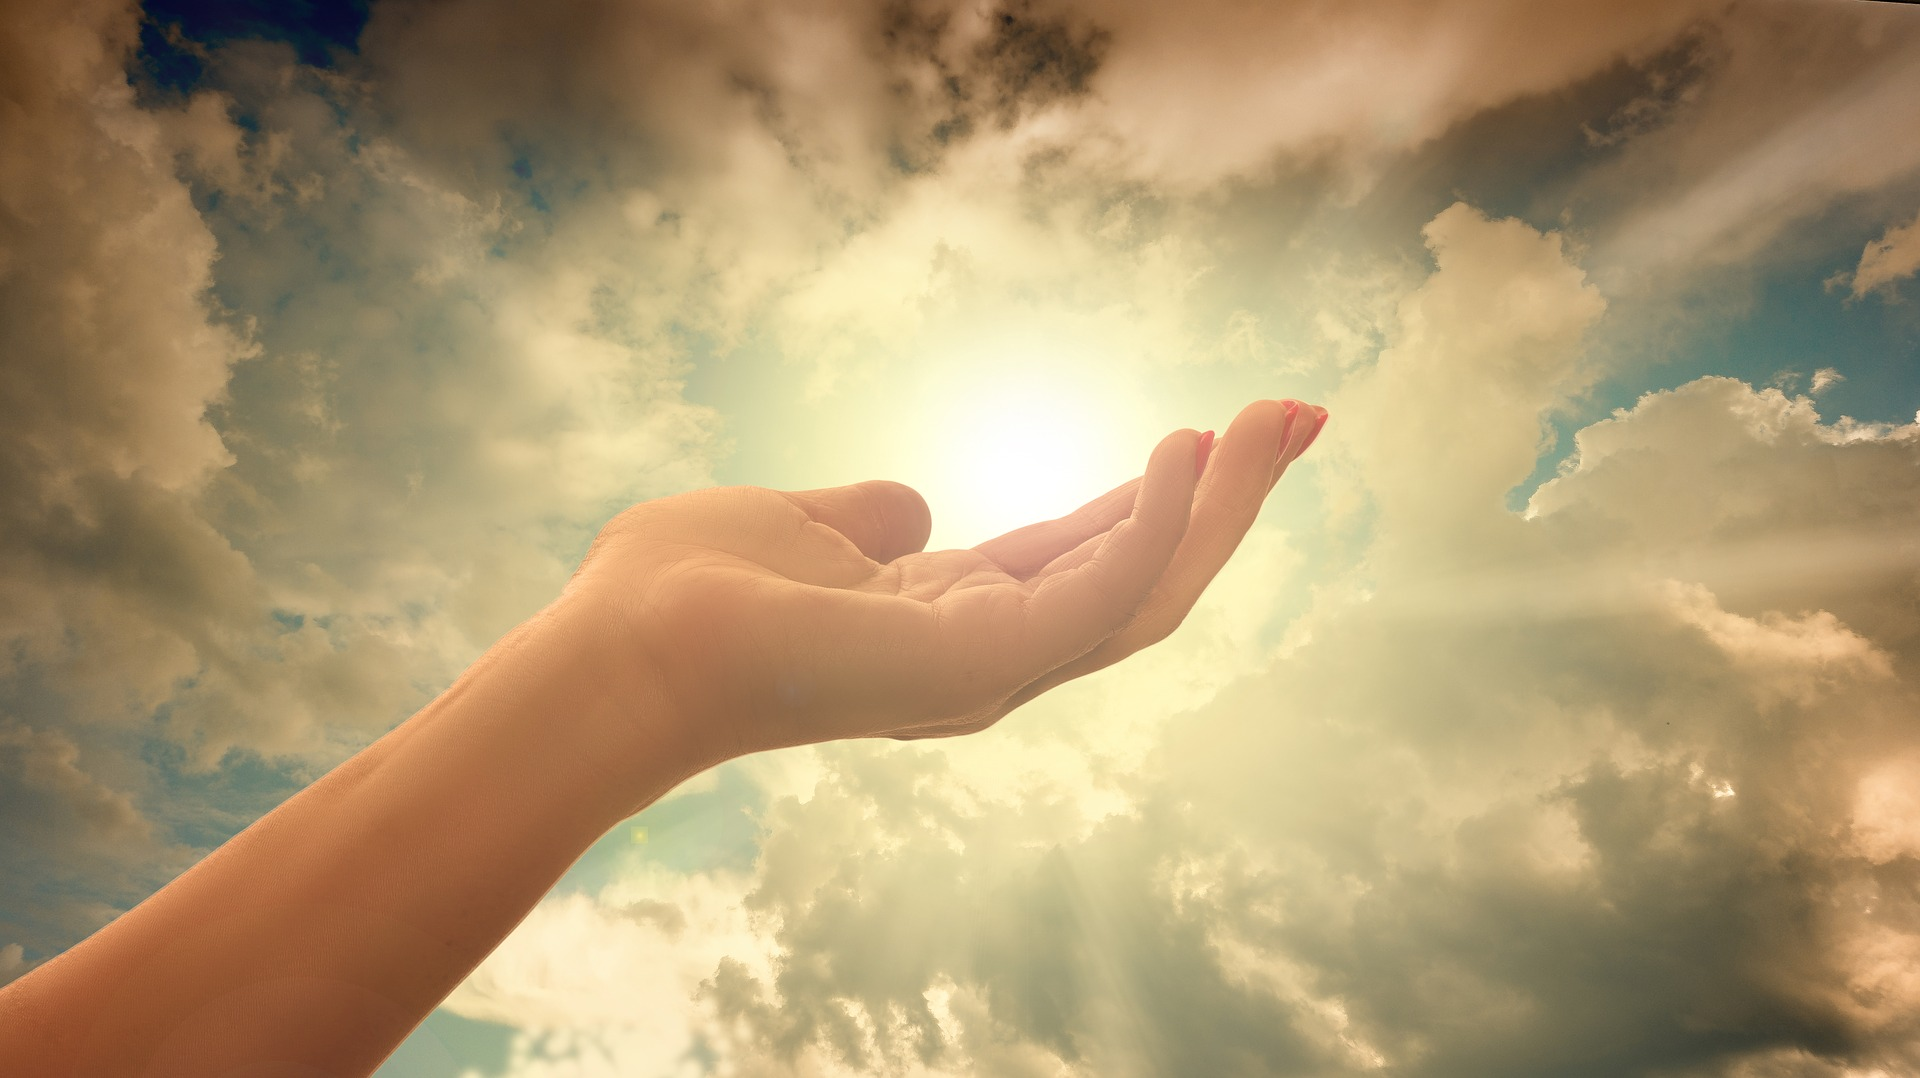
\includegraphics{religion-g96a8473e7_1920.jpg}

The idea behind this project originated with consideration of Aristotle's perspective regarding balance, specifically with regard to the ``golden mean''. This is a moral location between excess and deficiency.

Currently the project aims to develop a 360\(^{\circ}\) instrument that can be applied to leaders, which delivers feedback along leadership-relevant but philosophically- and spiritually-derived values and virtues.

\begin{itemize}
\tightlist
\item
  leadership-relevant
\item
  feedback focused
\item
  spiritual and philosophical derivation
\end{itemize}

\hypertarget{literature}{%
\chapter{Literature}\label{literature}}

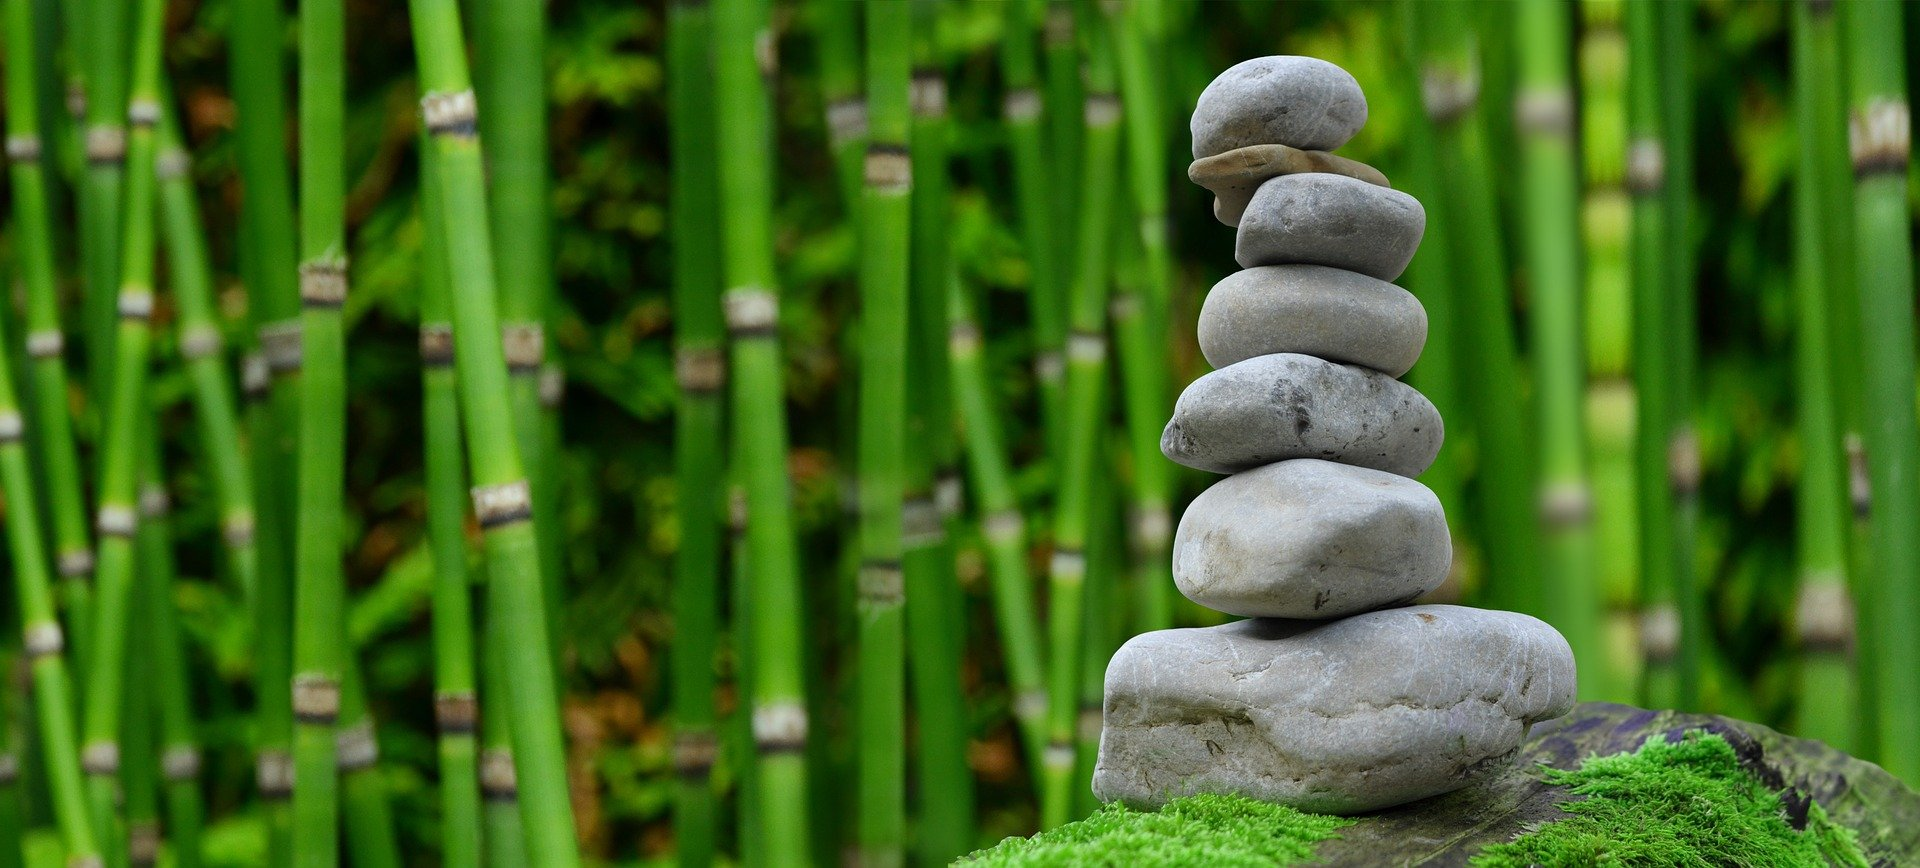
\includegraphics{stones-ge8c321976_1920.jpg}

Here is a review of sources considered:

\hypertarget{methods}{%
\chapter{Methods}\label{methods}}

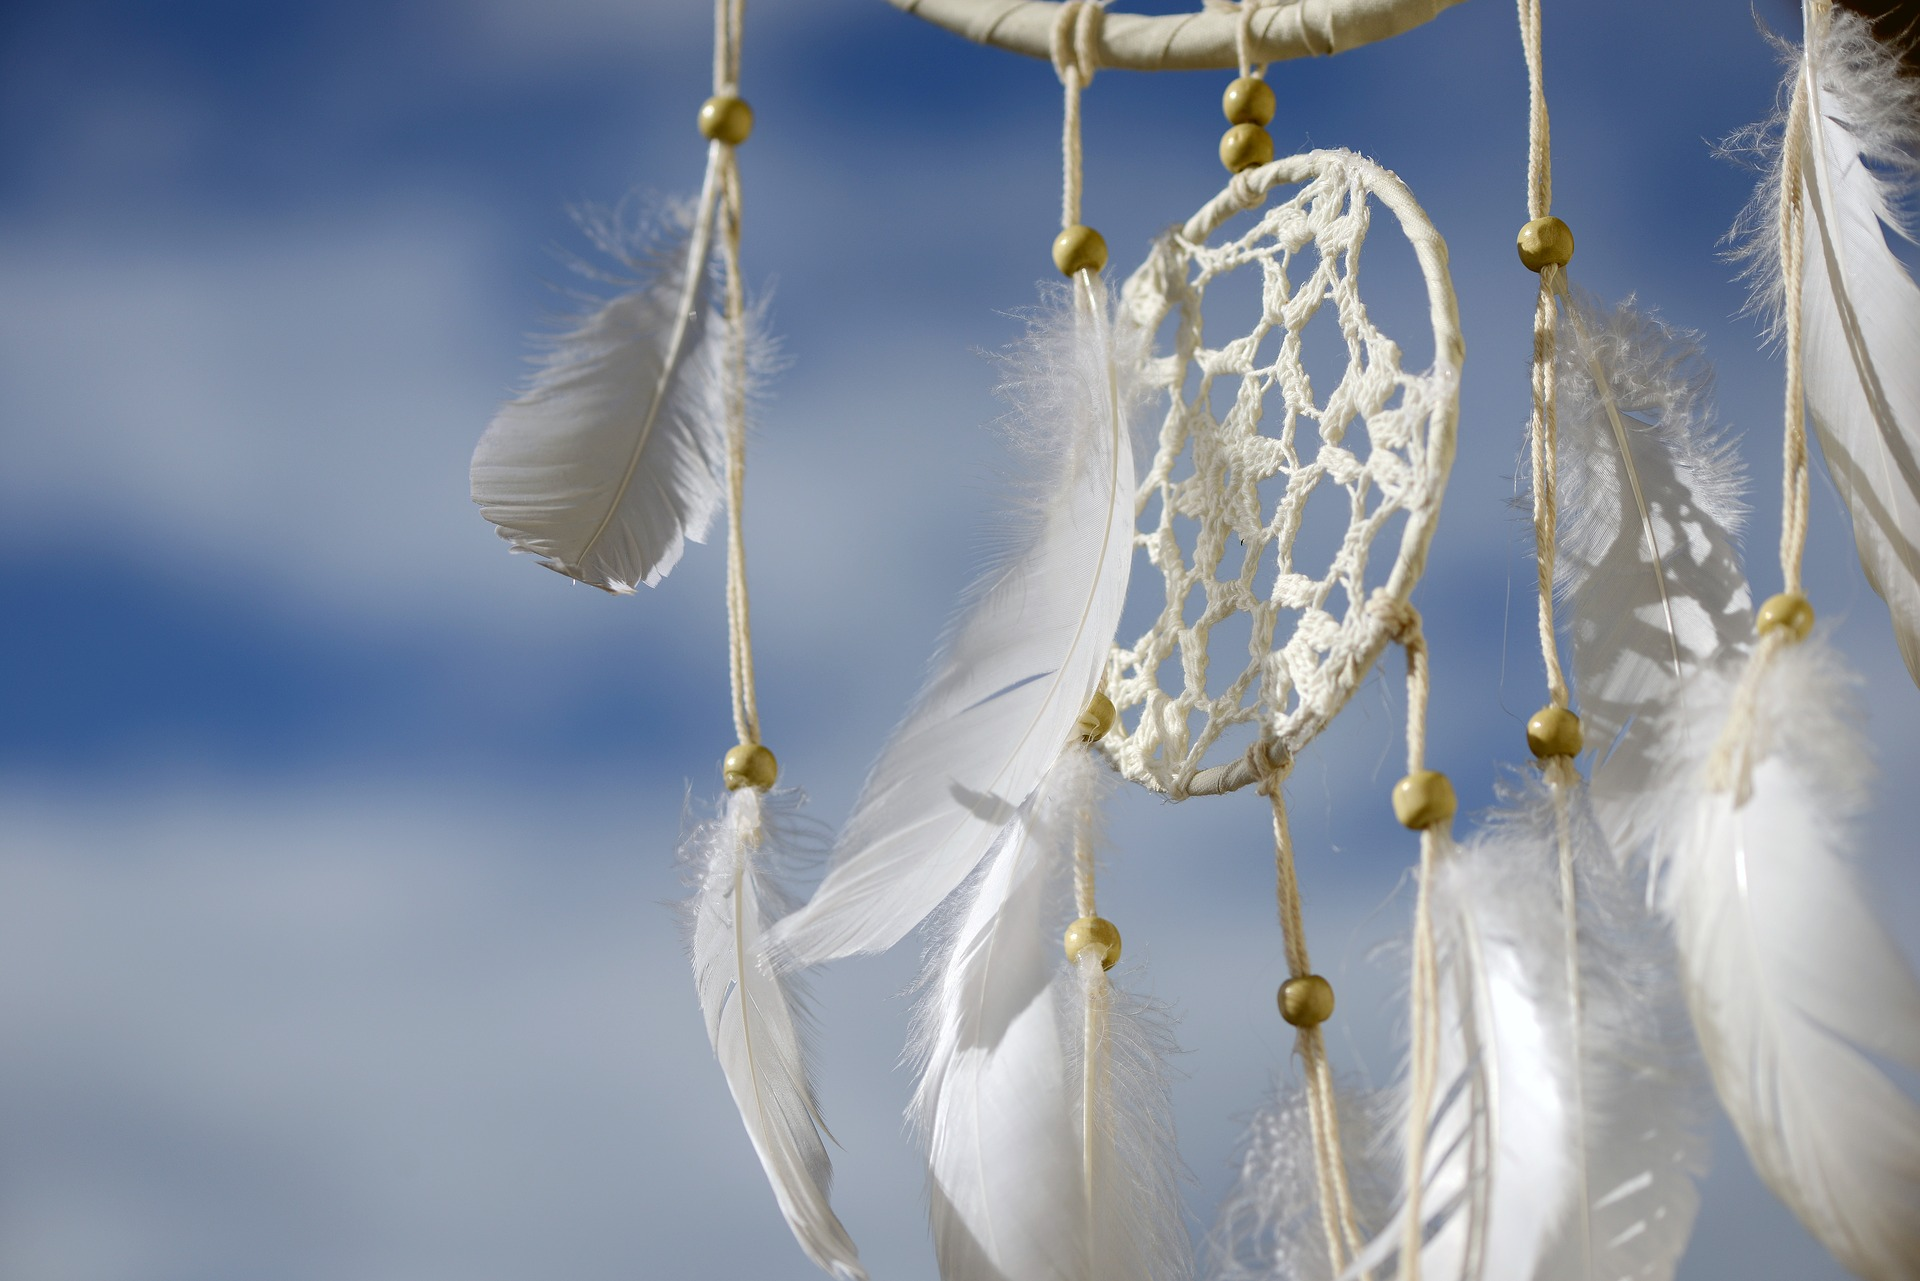
\includegraphics{dream-catcher-g6ec41bb43_1920.jpg}

We describe our methods regarding instrument development in this chapter.

\hypertarget{results}{%
\chapter{Results}\label{results}}

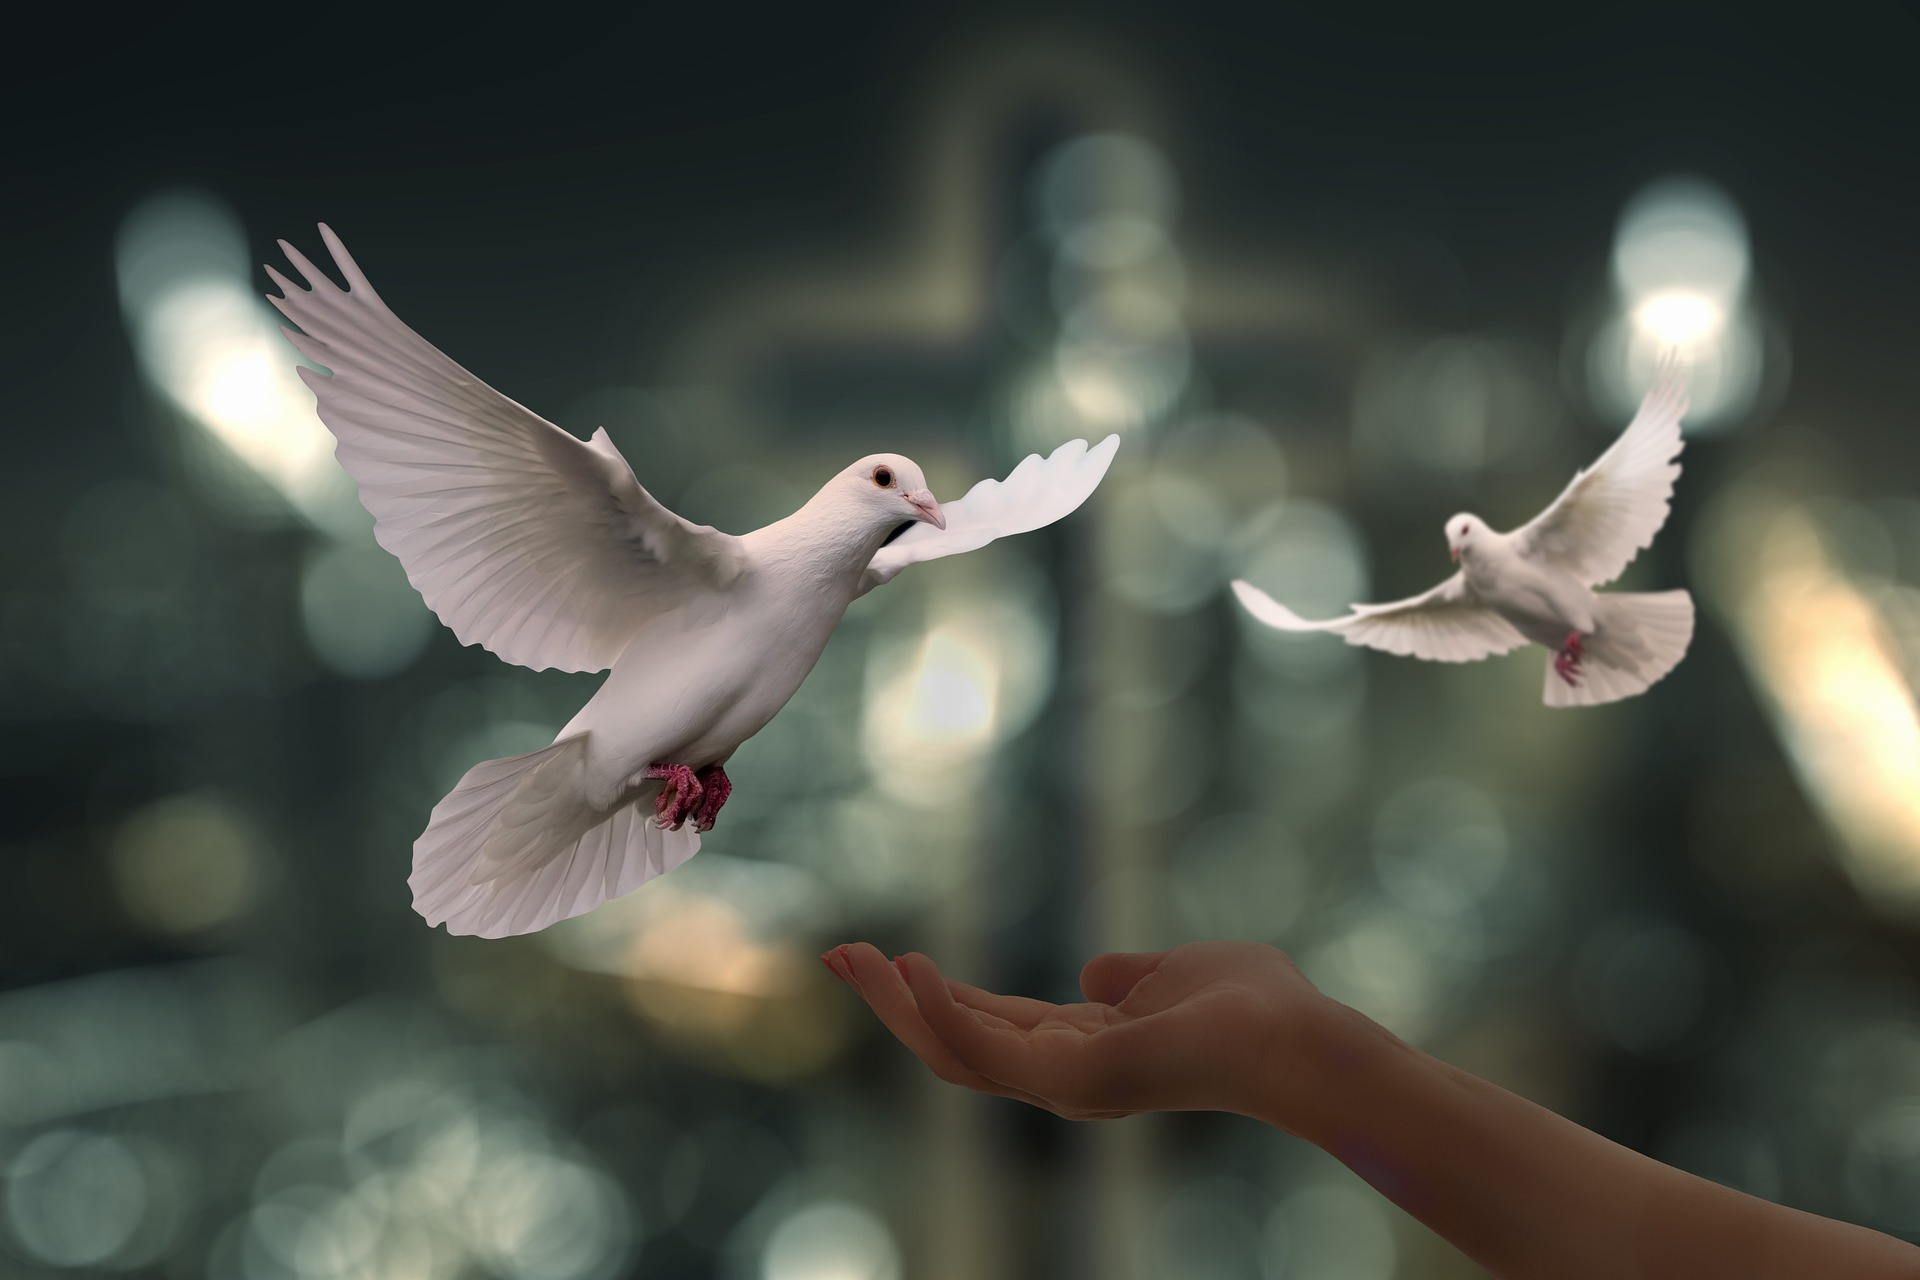
\includegraphics{doves-g750d44923_1920.jpg}

\hypertarget{content-validation}{%
\section{Content Validation}\label{content-validation}}

\hypertarget{pilot-administration}{%
\section{Pilot Administration}\label{pilot-administration}}

\hypertarget{construct-and-criterion-related-validation}{%
\section{Construct and Criterion-related Validation}\label{construct-and-criterion-related-validation}}

\hypertarget{future-directions}{%
\chapter{Future Directions}\label{future-directions}}

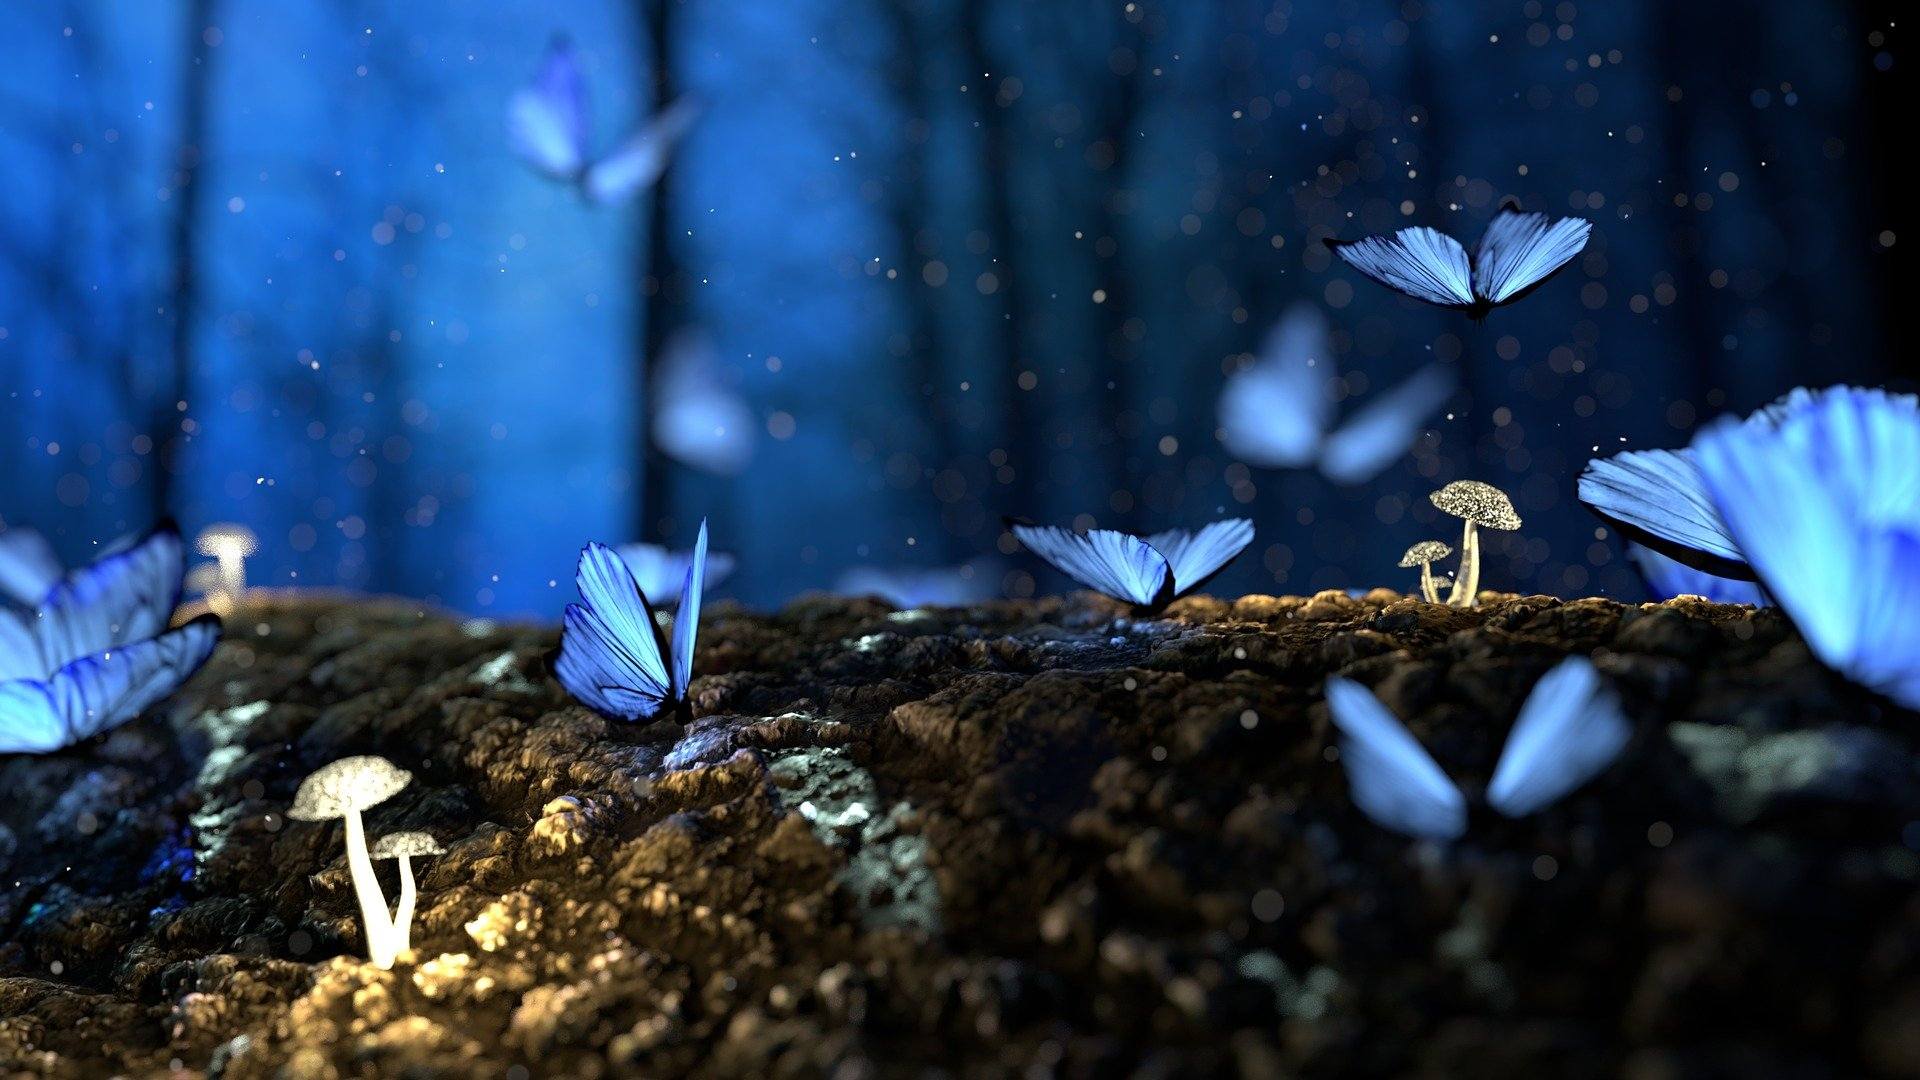
\includegraphics{fantasy-g653fba516_1920.jpg}

Now we're famous.

  \bibliography{book.bib,packages.bib}

\end{document}
